\documentclass[nofonts]{beamer}

\usepackage[UTF8, noindent]{ctexcap}
\usepackage{tikz}
\usetheme{PaloAlto}

% 设置中文字体
\setCJKmainfont{AR PL UMing CN}
\setCJKsansfont{AR PL UMing CN}
\setCJKmonofont{WenQuanYi Micro Hei Mono}

% 设置英文字体
\setmainfont{Times New Roman}
\setsansfont{Droid Sans Mono}
\setmonofont{FreeMono}

\begin{document}
\begin{frame}
	\begin{center}
		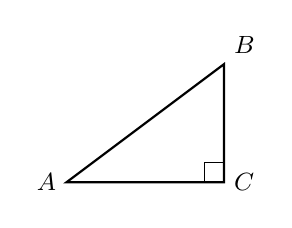
\begin{tikzpicture}[scale=0.5, font=\small]
			\draw[thick] (0, 0) node[left] {$A$}
			-- (4, 0) node[right] {$C$}
			-- (4, 3) node[above right] {$B$} -- cycle;
			\draw (3.5, 0) |- (4, 0.5);
		\end{tikzpicture}
	\end{center}
\end{frame}
\end{document}
